\contourlength{1.0pt}

\tikzset{>=latex} % for LaTeX arrow head
\colorlet{myblue}{blue!65!black}
\colorlet{mydarkblue}{blue!50!black}
\colorlet{myred}{red!65!black}
\colorlet{mydarkred}{red!40!black}
\colorlet{veccol}{green!70!black}
\colorlet{vcol}{green!70!black}
\colorlet{xcol}{blue!85!black}
\tikzstyle{vector}=[->,very thick,xcol,line cap=round]
\tikzstyle{xline}=[myblue,very thick]
\tikzstyle{yzp}=[canvas is zy plane at x=0]
\tikzstyle{xzp}=[canvas is xz plane at y=0]
\tikzstyle{xyp}=[canvas is xy plane at z=0]
\def\tick#1#2{\draw[thick] (#1) ++ (#2:0.12) --++ (#2-180:0.24)}
\def\N{100}

% COMPLEX




% COMPLEX numbers


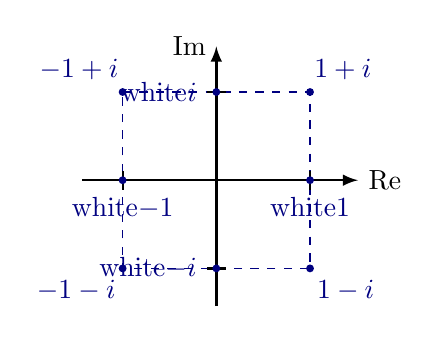
\begin{tikzpicture}
  \def\xmax{1.7}
  \def\ymax{1.6}
  \def\re{0.7*\xmax}
  \def\im{0.7*\ymax}
  \coordinate (O) at (0,0);
  \draw[dashed,mydarkblue]
    (-\re,\im) -| (\re,-\im) -| cycle;
  \draw[->,line width=0.9] (-\xmax,0) -- (\xmax+0.1,0) node[right] {Re};
  \draw[->,line width=0.9] (0,-\ymax) -- (0,\ymax+0.1) node[left] {Im};
  \tick{\re,0}{90} node[mydarkblue,scale=1,below=-1] {\contour{white}{$1$}};
  \tick{-\re,0}{90} node[mydarkblue,scale=1,below=-1] {\contour{white}{$-1$}};
  \tick{0,\im}{ 0} node[mydarkblue,scale=1,left] {\contour{white}{$i$}}; %r\sin\theta = 
  \tick{0,-\im}{ 0} node[mydarkblue,scale=1,left] {\contour{white}{$-i$}};
  \fill[mydarkblue]
    (   0, \im) circle(0.05)
    (   0,-\im) circle(0.05)
    ( \re,   0) circle(0.05)
    (-\re,  0) circle(0.05)
    ( \re, \im) circle(0.05)
      node[mydarkblue,scale=1,above right=-2] {\strut$1+i$}
    ( \re,-\im) circle(0.05)
      node[mydarkblue,scale=1,below right=-1] {\strut$1-i$}
    (-\re, \im) circle(0.05)
      node[mydarkblue,scale=1,above left=-2] {\strut$-1+i$}
    (-\re,-\im) circle(0.05)
      node[mydarkblue,scale=1,below left=-1] {\strut$-1-i$};
\end{tikzpicture}
